
\section{Similar solutions}

	\subsection{Parallel Kingdom - Age of Ascension}
	This game was on market for 8 years (2008-2016). Parallel Kingdom is a closest solution to ours.
	
	
	”Parallel Kingdom is a mobile, location based, massively multiplayer game that uses GPS
	location and Google Maps to place users in a virtual world. Parallel Kingdom is the first
	location based RPG for the iOS and Android platforms. The game is set in a virtual world
	or ”Parallel Kingdom” where users claim their territories based on their GPS location or by making friends who invite them to travel to new places. Parallel Kingdom is a freemium
	game and utilizes a virtual goods revenue model.”
	
	\subsection{Ingress}
	Developed by Niantic, which was then part of Google, this game was released in 2013 for
	Android and in 2014 for iOS.[4] It is a location based, massively multiplayer game. A player have to choose one of the two factions, Enlightened or Resistance, and then as a part of his 	team capture regions of the game map. A faith of each faction relies on players’ cooperation. Thanks to that players meet in real life and coordinate their actions.
	
	Ingress was the first very successful augmented reality game with more than 10 000 000
	installs.
	
	\subsection{Pokémon GO}
	After its success with Ingress, Niantic started working on a new game Pokemon GO. Once
	released, the game became incredible hit. Even though the game faced many problems during
	its launch, mainly caused by the unexpected success and more active users than Pokémon
	GO was able to handle, in the first 80 days Pokémon GO reached about 550 million downloads and earned about \$470 million.
	
	The game is very similar to Ingress and uses the same crowd-sourced geographical data.
	
\section{Use Cases}

	\subsection{Use case diagram}
	
		\begin{figure}[h]	
			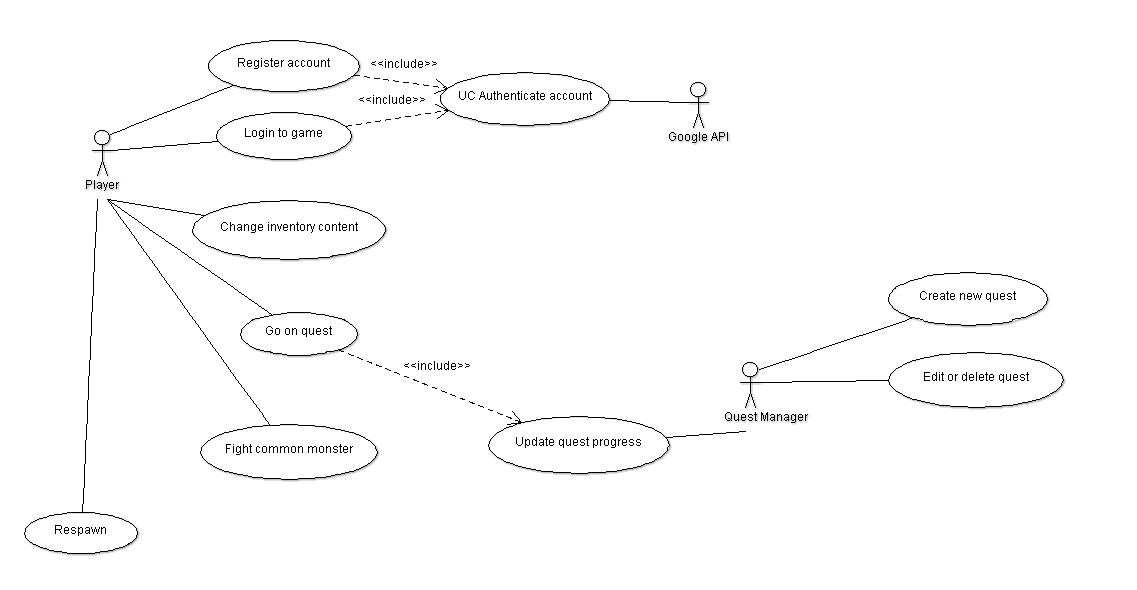
\includegraphics[width=\textwidth]{figures/UseCaseDiagram}
			\centering			
			\caption{Use case diagram}
			\label{fig:usecasediagram}
		\end{figure}
	
	\subsection{Use case descriptions}
		The following section refer to the use-cases introduced in Figure \ref{fig:usecasediagram}.
		\begin{enumerate}
			\item \textbf{Register account} \\
			\item \textbf{Login to the game} \\
			\item \textbf{Change the inventory content} \\
			\item \textbf{Go on a quest} \\
			\item \textbf{Fight a common monster} \\
			\item \textbf{Respawn} \\
			\item \textbf{Update a quest progress} \\
			\item \textbf{Create a new quest} \\
			\item \textbf{Edit or delete a quest} \\
						
		\end{enumerate}
	
	
\section{Requirements}

	\subsection{Functional}
		\begin{enumerate}
			\item \textbf{Users can use their Google accounts to login and play} \\
			For player's convenience, a Google account is required to play. The application does not have to store any password. 
			
			\item \textbf{Client can request nearby game locations} \\
			Upon client's request, the server has to respond with all game locations near the position of the client. The request can contain a filter.
			
			\item \textbf{Client can add, delete and update the player's inventory} \\
		\end{enumerate}
		
		
	\subsection{Non-functional}
	
		\begin{enumerate}
			\item \textbf{The data layer consists of a database engine and a caching} \\
			Game Server never accesses database directly. Data are retrieved from the database upon request and then cached. Upper layers communicate exclusively with cache.		
			
			\item \textbf{The server provides an API for client} \\
			The API support at least following:
			\begin{enumerate}
				\item Retrieve nearby game locations
				\item Create player
				\item Update player's data (inventory, experience, resources, quests progress etc.)
				\item Provide information about a quest 			
			\end{enumerate}
			
			\item \textbf{The communication between client and server parts of the application must be secure} \\
			All data sent from and to a client has to be encrypted.
	
			\item \textbf{Client can only connect to a Connection Server} \\
			Several Connection Servers exist to prevent a bottle-neck. Client selects the Connection Server by an algorithm. Client does not have an access to any other part of the server.
		\end{enumerate}
	\subsection{System and Interface}
	
		\begin{enumerate}
			\item \textbf{System uses Java 8 SE as an execution environment} \\
			
			\item \textbf{Operating system for the server is Debian 8} \\
			
			\item \textbf{Database engine is MySQL} \\
			
			\item \textbf{Cache engine is Redis} \\
		\end{enumerate}
	
\section{Technology}

	\subsection{Frameworks}
	